\documentclass[border=15pt, multi, tikz]{standalone}
\usepackage{import}
\subimport{../../layers/}{init}
\usetikzlibrary{positioning}
\usetikzlibrary{3d} %for including external image

\def\ConvColor{rgb:yellow,5;red,2.5;white,5}
\def\ConvReluColor{rgb:yellow,5;red,5;white,5}
\def\PoolColor{rgb:red,1;black,0.3}
\def\DcnvColor{rgb:blue,5;green,2.5;white,5}
\def\SoftmaxColor{rgb:magenta,5;black,7}
\def\SumColor{rgb:blue,5;green,15}
\def\poolsep{1}
\def\FcColor{rgb:blue,5;red,2.5;white,5}
\def\FcReluColor{rgb:blue,5;red,5;white,4}

\begin{document}
\begin{tikzpicture}
\tikzstyle{connection}=[ultra thick,every node/.style={sloped,allow upside down},draw=\edgecolor,opacity=0.6]
%%%%%%%%%%%%%%%%%%%%%%%%%%%%%%%%%%%%%%%%%%%%%%%%%%%%%%%%%%%%%%%%%%%%%%%%%%%%%%%%%%%%%%%%
%% Draw Layer Blocks
%%%%%%%%%%%%%%%%%%%%%%%%%%%%%%%%%%%%%%%%%%%%%%%%%%%%%%%%%%%%%%%%%%%%%%%%%%%%%%%%%%%%%%%%
\node[canvas is zy plane at x=0] (temp) at (-3,0,0) {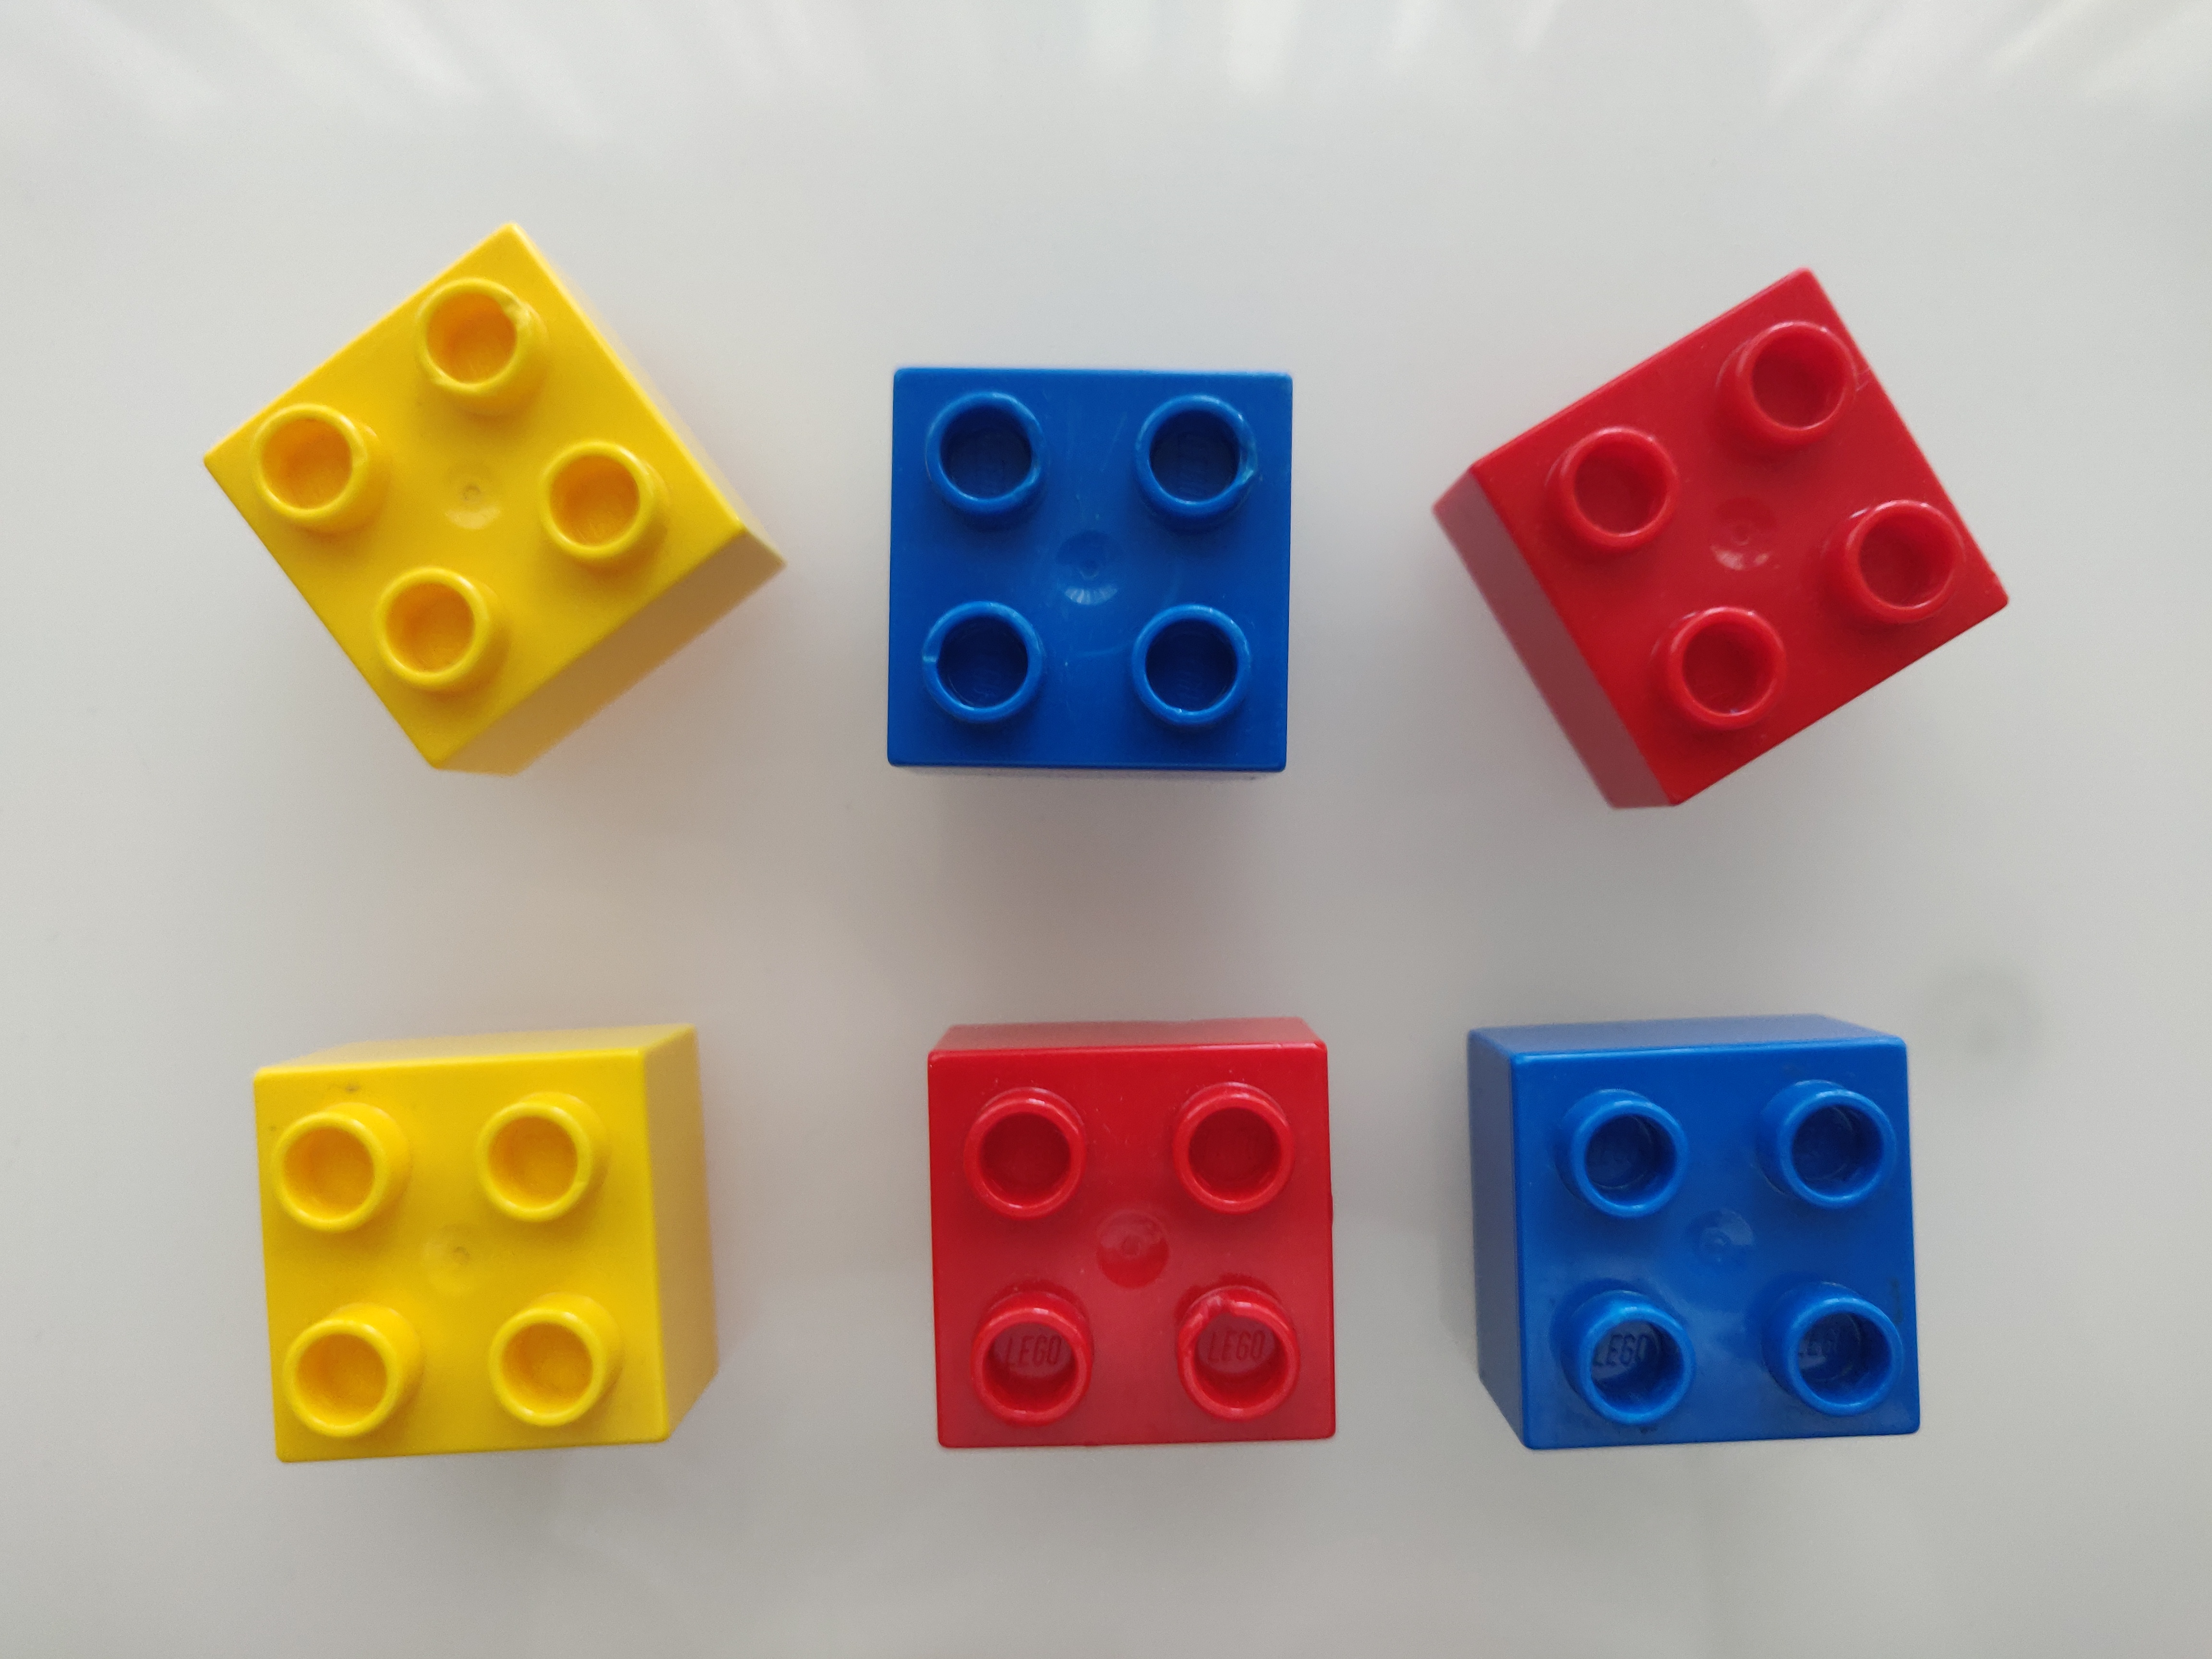
\includegraphics[width=8cm,height=8cm]{LEGO.jpg}};

% conv1_1,conv1_2,%pool1
\pic[shift={(0,0,0)}] at (0,0,0) {RightBandedBox={name=cr1,caption=conv1,
        xlabel={{"",""}},zlabel=,fill=\ConvColor,bandfill=\ConvReluColor,%
        height=40,width={2,2},depth=40}};
\pic[shift={(0,0,0)}] at (cr1-east) {Box={name=p1,%
        fill=\PoolColor,opacity=0.5,height=30,width=1,depth=30}};
%%%%%%%%%%

% conv2_1,conv2_2,pool2
\pic[shift={(1,0,0)}] at (p1-east) {RightBandedBox={name=cr2,caption=conv2,
        xlabel={{"",""}},ylabel=,zlabel=,fill=\ConvColor,bandfill=\ConvReluColor,%
        height=30,width={3,3},depth=30}};
\pic[shift={(0,0,0)}] at (cr2-east) {Box={name=p2,%
        fill=\PoolColor,opacity=0.5,height=23,width=1,depth=23}};
%%%%%%%%%%
 
% conv3_1,conv3_2,conv3_3,pool3
\pic[shift={(1,0,0)}] at (p2-east) {RightBandedBox={name=cr3,caption=conv3,
        xlabel={{"","",""}},ylabel=,zlabel=,fill=\ConvColor,bandfill=\ConvReluColor,%
        height=23,width={4,4,4},depth=23}};
\pic[shift={(0,0,0)}] at (cr3-east) {Box={name=p3,%
        fill=\PoolColor,opacity=0.5,height=14,width=1,depth=14}};
%%%%%%%%%%      

% conv4_1,conv4_2,conv4_3,pool4
\pic[shift={(1,0,0)}] at (p3-east) {RightBandedBox={name=cr4,caption=conv4,
        xlabel={{"","",""}},ylabel=,zlabel=,fill=\ConvColor,bandfill=\ConvReluColor,%
        height=14,width={7,7,7},depth=14}};
\pic[shift={(0,0,0)}] at (cr4-east) {Box={name=p4,%
        fill=\PoolColor,opacity=0.5,height=8,width=1,depth=8}};
%%%%%%%%%%

% conv5_1,conv5_2,conv5_3,pool5
\pic[shift={(1,0,0)}] at (p4-east) {RightBandedBox={name=cr5,caption=conv5,
        xlabel={{"","",""}},zlabel=,fill=\ConvColor,bandfill=\ConvReluColor,%
        height=8,width={7,7,7},depth=8}};
\pic[shift={(19,0,0)}] at (cr5-east) {Box={name=p5,%
        fill=\PoolColor,opacity=0.5,height=6,width=1,depth=6}};
%%%%%%%%%%
        
% fc6
\pic[shift={(2,0,0)}] at (p5-east) {RightBandedBox={name=fc6,caption=fc6,%
        xlabel={{"",""}},ylabel=,zlabel=,fill=\FcColor,bandfill=\FcReluColor,%
        height=3,width=3,depth=100}};
%%%%%%%%%%

% fc7
\pic[shift={(2,0,0)}] at (fc6-east) {RightBandedBox={name=fc7,caption=fc7,%
        xlabel={{"","dummy"}},ylabel=,zlabel=,fill=\FcColor,bandfill=\FcReluColor,%
        height=3,width=3,depth=100}};
%%%%%%%%%%

% fc8
\pic[shift={(3,0,0)}] at (fc7-east) {RightBandedBox={name=fc8,caption=rcnnfc+
softmax,%
        xlabel={{"","dummy"}},ylabel=,fill=\FcColor,bandfill=\FcReluColor,%
        height=3,width=3,depth=5}};
%%%%%%%%%%

% softmax
\pic[shift={(0,0,0)}] at (fc8-east) {Box={name=softmax,%
        xlabel={{"","dummy"}},zlabel=,opacity=0.8,fill=\SoftmaxColor,%
        height=3,width=1.5,depth=5}};


%%%%%%%%%%%%%%%%%%%%%%%%%%%%%%%%%%%%%%%%%%%%%%%%%%%%%%%%%%%%%%%%%%%%%%%%%%%%%%%%%%%%%%%%
\def\skipshift{12}
%%Joining with previous streams (fcn-16)
%% score8
\pic[shift={(4,0,\skipshift)}] at (cr5-east) {Box={name=score8,caption=rpnConv,
        xlabel={{"","dummy"}},fill=\ConvColor,height=14,width=4,depth=14,ylabel=,zlabel=}};
        
%%Joining with previous streams
%% score16_1
\pic[shift={(4,0,6)}] at (score8-east) {Box={name=score16_1,caption=rpnConv-BoxDeltas,
        xlabel={{"","dummy"}},fill=\ConvColor,height=14,width=2,depth=14,ylabel=,zlabel=}};
        
%%Joining with previous streams
%% score32_1
\pic[shift={(2,0,0)}] at (score16_1-east) {Box={name=score32_1,caption=rpnBoxDeltas,
        xlabel={{"","dummy"}},fill=\ConvColor,height=14,width=2,depth=14,ylabel=,zlabel=}};

%%Joining with previous streams
%% score16_2
\pic[shift={(4,0,-6)}] at (score8-east) {Box={name=score16_2,caption=rpnConv-ClsScores,
        xlabel={{"","dummy"}},fill=\ConvColor,height=14,width=2,depth=14,ylabel=,zlabel=}};
        
%%Joining with previous streams
%% score32_2
\pic[shift={(2,0,0)}] at (score16_2-east) {Box={name=score32_2,caption=rpnSoftmax,
        xlabel={{"","dummy"}},fill=\ConvColor,height=14,width=2,depth=14,ylabel=,zlabel=}};  
        
%%Joining with previous streams
%% score64_2
\pic[shift={(2,0,0)}] at (score32_2-east) {Box={name=score64_2,caption=rpnClassification,
        xlabel={{"","dummy"}},fill=\ConvColor,height=14,width=2,depth=14,ylabel=,zlabel=}};
        
%%Joining with previous streams
%% score64_3
\pic[shift={(13,0,0)}] at (score8-east) {Box={name=score64_3,caption=RegionProposal,
        xlabel={{"","dummy"}},fill=\ConvColor,height=14,width=2,depth=14,ylabel=,zlabel=}};      
        

%%%%%%%%%%%%%%%%%%%%%%%%%%%%%%%%%%%%%%%%%%%%%%%%%%%%%%%%%%%%%%%%%%%%%%%%%%%%%%%%%%%%%%%%%
%%Joining with previous streams (fc7)
%% aux8
\pic[shift={(3,0,7)}] at (fc7-east) {RightBandedBox={name=aux8,caption=fc+BoxDeltas,%
        xlabel={{"","dummy"}},ylabel=,fill=\FcColor,bandfill=\FcReluColor,%
        height=3,width=3,depth=5}};
%%%%%%%%%%

% boxdeltas
\pic[shift={(0,0,0)}] at (aux8-east) {Box={name=boxdeltas,%
        xlabel={{"","dummy"}},zlabel=,opacity=0.8,fill=\SoftmaxColor,%
        height=3,width=1.5,depth=5}};



%%%%%%%%%%%%%%%%%%%%%%%%%%%%%%%%%%%%%%%%%%%%%%%%%%%%%%%%%%%%%%%%%%%%%%%%%%%%%%%%%%%%%%%%
%%% Draw connections
%%%%%%%%%%%%%%%%%%%%%%%%%%%%%%%%%%%%%%%%%%%%%%%%%%%%%%%%%%%%%%%%%%%%%%%%%%%%%%%%%%%%%%%%%
\draw [connection]  (p1-east)    -- node {\midarrow} (cr2-west);
\draw [connection]  (p2-east)    -- node {\midarrow} (cr3-west);
\draw [connection]  (p3-east)    -- node {\midarrow} (cr4-west);
\draw [connection]  (p4-east)    -- node {\midarrow} (cr5-west);
\draw [connection]  (cr5-east)    -- node {\midarrow} (p5-west);
%

\path (cr5-east) -- (p5-west) coordinate[pos=0.1] (after4) ;
\draw [connection]  (after4)    -- node {\midarrow} ++(0,0,\skipshift) -- node {\midarrow} (score8-west);

\draw [connection]  (score8-east)   -- node {\midarrow} ++(1.95,0,0);
\path (score8-east) -- (score64_3-west) coordinate[pos=0.15] (after5) ;
\draw [connection]  (after5)    -- node {\midarrow} ++(0,0,6) -- node {\midarrow} (score16_1-west);
\draw [connection]  (after5)    -- node {\midarrow} ++(0,0,-6) -- node {\midarrow} (score16_2-west);

\draw [connection]  (score16_1-east)    -- node {\midarrow} (score32_1-west);
\draw [connection]  (score32_1-east)   -- node {\midarrow} ++(1.5,0,0);
\draw [connection]  (score16_2-east)    -- node {\midarrow} (score32_2-west);
\draw [connection]  (score32_2-east)    -- node {\midarrow} (score64_2-west);
\draw [connection]  (score64_2-east)   -- node {\midarrow} ++(1.5,0,0);

\path (score16_1-east) -- (score32_1-west) coordinate[pos=0.2] (after5) ;
\draw [connection]  (after5)    -- node {\midarrow} ++(0,0,-6) -- node {\midarrow} (score64_3-west);

\path (score16_2-east) -- (score32_2-west) coordinate[pos=0.2] (after6) ;
\draw [connection]  (after6)    -- node {\midarrow} ++(0,0,+6) -- node {\midarrow} (score64_3-west);

\path (score64_3-east) -- (p5-west) coordinate[pos=0] (after7) ;
\draw [connection]  (after7)    -- node {\midarrow} ++(1,0,0) -- node {\midarrow} (p5-west);


\draw [connection]  (p5-east)    -- node {\midarrow} (fc6-west);
\draw [connection]  (fc6-east)       -- node {\midarrow} (fc7-west);
\draw [connection]  (fc7-east)       -- node {\midarrow} (fc8-west);
\draw [connection]  (softmax-east)   -- node {\midarrow} ++(1.5,0,0);

\path (fc7-east) -- (fc8-west) coordinate[pos=0.4] (after8) ;
\draw [connection]  (after8)    -- node {\midarrow} ++(0,0,7) -- node {\midarrow} (aux8-west);
\draw [connection]  (boxdeltas-east)   -- node {\midarrow} ++(1.5,0,0);

%%%%%%%%%%%%%%%%%%%%%%%%%%%%%%%%%%%%%%%%%%%%%%%%%%%%%%%%%%%%%%%%%%%%%%%%%%%%%%%%%%%%%%%%

\end{tikzpicture}
\end{document}\grid
